\RequirePackage[l2tabu,orthodox]{nag} % warn if using any obsolete commands
\documentclass[12pt,letterpaper]{article} % document style

% load encoding and font packages for pdflatex, in order
\usepackage[T1]{fontenc} % output 8-bit encoded fonts
\usepackage[utf8]{inputenc} % allow input of utf-8 encoded characters
\usepackage{ebgaramond} % document's serif font
\usepackage{tgheros} % document's sans serif font

% load babel, csquotes, and microtype in order
\usepackage[USenglish]{babel} % auto-regionalize hyphens, quote marks, etc
\usepackage[strict,autostyle]{csquotes} % smart and nestable quote marks
\usepackage[babel=true]{microtype} % enable micro-typographic adjustments

% load everything else
\usepackage{amsmath} % additional mathematical typesetting features
\usepackage{authblk} % footnote-style author/affiliation info
\usepackage{booktabs} % better looking tables
\usepackage{caption} % custom figure/table caption styles
\usepackage{datetime} % enable formatting of date output
\usepackage[final]{draftwatermark} % watermark paper as a draft
\usepackage{endnotes} % enable endnotes
\usepackage{geometry} % configure page dimensions and margins
\usepackage{graphicx} % better inclusion of graphics
\usepackage{natbib} % textual/parenthetical author-year citations w/bibtex
\usepackage{pdflscape} % rotate wide tables/figures to make them landscape
\usepackage{setspace} % configure spacing between lines
\usepackage{titlesec} % custom section and subsection heading
\usepackage{url} % make nice line-breakable urls

% load hyperref/orcidlink last for compatibility
\usepackage{hyperref} % enable hyperlinks and pdf metadata
\usepackage{orcidlink} % provide orcid logo and link

% print only the month and year when using \today
\newdateformat{monthyeardate}{\monthname[\THEMONTH] \THEYEAR}

\newcommand{\myname}{Geoff Boeing}
\newcommand{\myorcid}{0000-0003-1851-6411}  % chktex 8
\newcommand{\myaffiliation}{Department of Urban Planning and Spatial Analysis\\University of Southern California}
\newcommand{\paperdate}{\monthyeardate\today}
\newcommand{\papertitle}{A City Is Sometimes Kind of a Tree: Urban Street Network Treeness and Constrained Redundancy}
\newcommand{\papercitation}{Boeing, G. \the\year{}. \papertitle. Under review at \textit{Journal Name}.}
\newcommand{\paperkeywords}{Urban Planning, Transportation, Data Science}

% location of figure files, via graphicx package
\graphicspath{{.}}

% configure the page layout, via geometry package
\geometry{
    paper=letterpaper, % paper size
    top=3.8cm, % margin sizes
    bottom=3.8cm,
    left=4cm,
    right=4cm}
\setstretch{1} % line spacing
\clubpenalty=10000 % prevent orphans
\widowpenalty=10000 % prevent widows

% set section/subsection headings as the sans serif font, via titlesec package
\titleformat{\section}{\normalfont\sffamily\large\bfseries\color{black}}{\thesection.}{0.3em}{}
\titleformat{\subsection}{\normalfont\sffamily\small\bfseries\color{black}}{\thesubsection.}{0.3em}{}
\titleformat{\subsubsection}{\normalfont\sffamily\small\color{black}}{\thesubsubsection.}{0.3em}{}

% make figure/table captions sans-serif small font
\captionsetup{font={footnotesize,sf},labelfont=bf,labelsep=period}

% configure pdf metadata and link handling, via hyperref package
\hypersetup{
    pdfauthor={\myname},
    pdftitle={\papertitle},
    pdfsubject={\papertitle},
    pdfkeywords={\paperkeywords},
    pdffitwindow=true, % window fit to page when opened
    breaklinks=true, % break links that overflow horizontally
    colorlinks=false, % remove link color
    pdfborder={0 0 0} % remove link border
}

\begin{document}

\title{\papertitle}%\footnote{Preprint of: \papercitation}}
\author[]{\myname~\orcidlink{\myorcid}}
\affil[]{\myaffiliation}
\date{\paperdate}

\maketitle

\begin{abstract}

Urban street network redundancy provides alternatives and resilience, but requires additional infrastructure and cost. This study develops the concept of \enquote{treeness}---how closely a network resembles a minimal version of itself stripped of all redundancy---to formally measure how cities have evolved or been designed to balance this trade-off. It defines two indicators of treeness---link redundancy and length redundancy---which compare each full street network to its minimum spanning tree, then calculates them for every urban area in the world. It finds that every urban street network is more tree-like than the baseline social and transport networks considered here, and that urban treeness varies surprisingly little around the world despite cities' diverse histories, sizes, and geographies. These findings suggest that street networks share a common balance between infrastructure cost and structural redundancy, constraining urban form while shaping resilience and vulnerability. Finally, we consider what this means for how we plan cities for more connected, sustainable futures.

\end{abstract}

\section{Introduction}

Redundancy in urban street networks comes with a trade-off. On one hand, it provides options, alternatives, and thus resilience to disruption \citep{boeing_2024_resilient}. On the other hand, redundancy requires duplicative infrastructure and thus higher capital and maintenance costs \citep{barthelemy_2022_spatial,cardillo_2006_structural}. This trade-off constrains how we build cities and shapes the resulting urban form. As policymakers increasingly emphasize connected, sustainable urbanization practices, the concept of \enquote{treeness}---how closely a network resembles a minimal version of itself stripped of all redundancy---offers a formal method of measuring how cities have evolved or been designed to balance this trade-off.

This study measures urban treeness to ask: to what extent are cities' street networks tree-like? It defines two indicators of treeness---link redundancy and length redundancy---which it calculates for every urban area's street network in the world. We find that \textit{every} urban street network in the world is more tree-like than the other baseline networks we compare it to. We also find that urban treeness varies relatively little around the world. This suggests that cities of diverse histories, sizes, and geographies have converged on a typical balance for the real-world trade-offs between infrastructure networks' structural redundancy and cost.

The remainder of this article is organized as follows. First it introduces the theory of urban treeness and reviews the mathematical formalization of trees in graph theory. Next it explains our methods for measuring treeness across the world's urban street networks, including data sources, analyses, baselines, and robustness checks. Then it presents our findings on urban treeness and its statistical and geographical distributions. Finally it discusses the implications of these findings for theorizing urban form and function and for planning more connected, sustainable cities.

\section{Theory}

\subsection{A City Is Not a Tree}

In 1965, design theorist Christopher Alexander wrote a short paper provocatively titled \enquote{A City Is Not a Tree} \citep{alexander_city_1965}. In it, he argued that urban planners---working centrally and top-down---tend to envision and design cities as hierarchical tree-like structures, whereas successful traditional cities evolve naturally as semi-lattices. That is, over-planned cities' street networks, neighborhoods, and school districts organize into hierarchical branching structures rather than interconnected lattices. The former implies efficiency and functional segregation. The latter implies \enquote{messy} interconnectedness and complexity. Alexander's claim was at once both descriptive and normative: (successful) cities \textit{are} not trees, and planners \textit{should} not plan cities as trees.

This paper became an influential landmark across urban studies and presaged complexity science's subsequent applications to cities \citep{rauber_alexanders_2018,huang_city_2022}. Alexander's argument dovetailed with the findings of emerging spatial network science that linked urban accessibility and resilience to interconnectedness and complexity in urban form \citep{jiang_complex-network_2016,park_network_2015}. However, Alexander adopted the language of \enquote{trees} metaphorically, merely gesturing at the mathematical definition of trees, let alone measuring whether a city actually is one empirically \citep{harary_city_1976}. Yet mathematics does provide a precise formalization of trees and their properties that allows us to model and measure cities---particularly their networks' redundancy and vulnerability---in useful ways.

\subsection{Network Treeness}\label{sec:theory_network_treeness}

Graph theory is the branch of discrete mathematics that studies networks \citep{trudeau_introduction_1994}. A graph, $G = (N, E)$ consists of a set of nodes, $N$, and a set of edges, $E$, that link pairs of nodes \citep{barthelemy_spatial_2011}. For example, we could model a street network as a spatial graph with nodes representing intersections/dead-ends and edges representing street segments, with both the nodes and the edges embedded in space \citep{fischer_spatial_2014,porta_2006_network}.

Formally, a tree is a type of graph that is connected and acyclic \citep{barthelemy_spatial_2011}. If $G$ is connected, then for all $u, v \in N$ there exists a sequence of edges that starts at $u$ and ends at $v$. And if $G$ is acyclic, then it contains no cycles, meaning there are no paths that start and end at the same node without retracing any edge. In other words, a tree contains exactly one path between any two nodes and every edge is a single point of failure \citep{newman_networks:_2010}. That is, if a connected graph $G$ contains $n = |N|$ nodes and $m = |E|$ edges, then $G$ is a tree if and only if $m = n - 1$, because the minimum number of edges needed to connect $n$ nodes is $n - 1$.

For our purposes, treeness entails two important properties for studying urban networks: redundancy and vulnerability \citep{barthelemy_2022_spatial}. Since a tree has only one path between any two nodes, if any edge is removed the network becomes disconnected. Accordingly trees have zero redundancy and are thus vulnerable to disruption (e.g., traffic congestion, collisions, floods, earthquakes, wildfires, terrorism) with no alternative routing options. In contrast, a less tree-like network offers multiple paths between nodes, providing redundancy and resilience to disruption when things go wrong \citep{barthelemy_spatial_2011}. Given these practical limitations of trees, one might expect that most cities evolved or were designed to incorporate at least some redundancy---which brings us to a graph-theoretic interpretation of Alexander's original metaphorical conjecture that cities are not trees.

One could empirically test this by measuring the treeness of a city's street network. For example, we could find the minimum spanning tree (MST) of the city's street network, and then compare it to the full network. Let $T$ be $G$'s MST: the tree that connects all of $G$'s nodes and minimizes total edge weight---e.g., total length in the case of urban streets \citep{barthelemy_2022_spatial}. We can calculate $T$'s total length, $L_T$, as:

\begin{equation}
    \label{eq:total_edge_length}
    L_T = \sum_{\{u, v\} \in E_T} \ell_{u, v}
\end{equation}

where $\ell_{u, v}$ is the length of the edge linking nodes $u$ and $v$, and $E_T$ is the edge set of $T$. Although the MST does not provide \enquote{last-step} access to the block frontages, it represents the minimal necessary infrastructure to preserve reachability across the network, thereby offering a theoretical lower bound and analytical counterfactual \citep{cardillo_2006_structural}. By comparing the full network modeled by $G$ to its MST $T$, we could measure how tree-like $G$ is by how much redundancy the street network contains beyond the minimal possible tree connecting all its nodes (\autoref{fig:network_examples}).

\begin{figure*}[tbh]
    \centering
    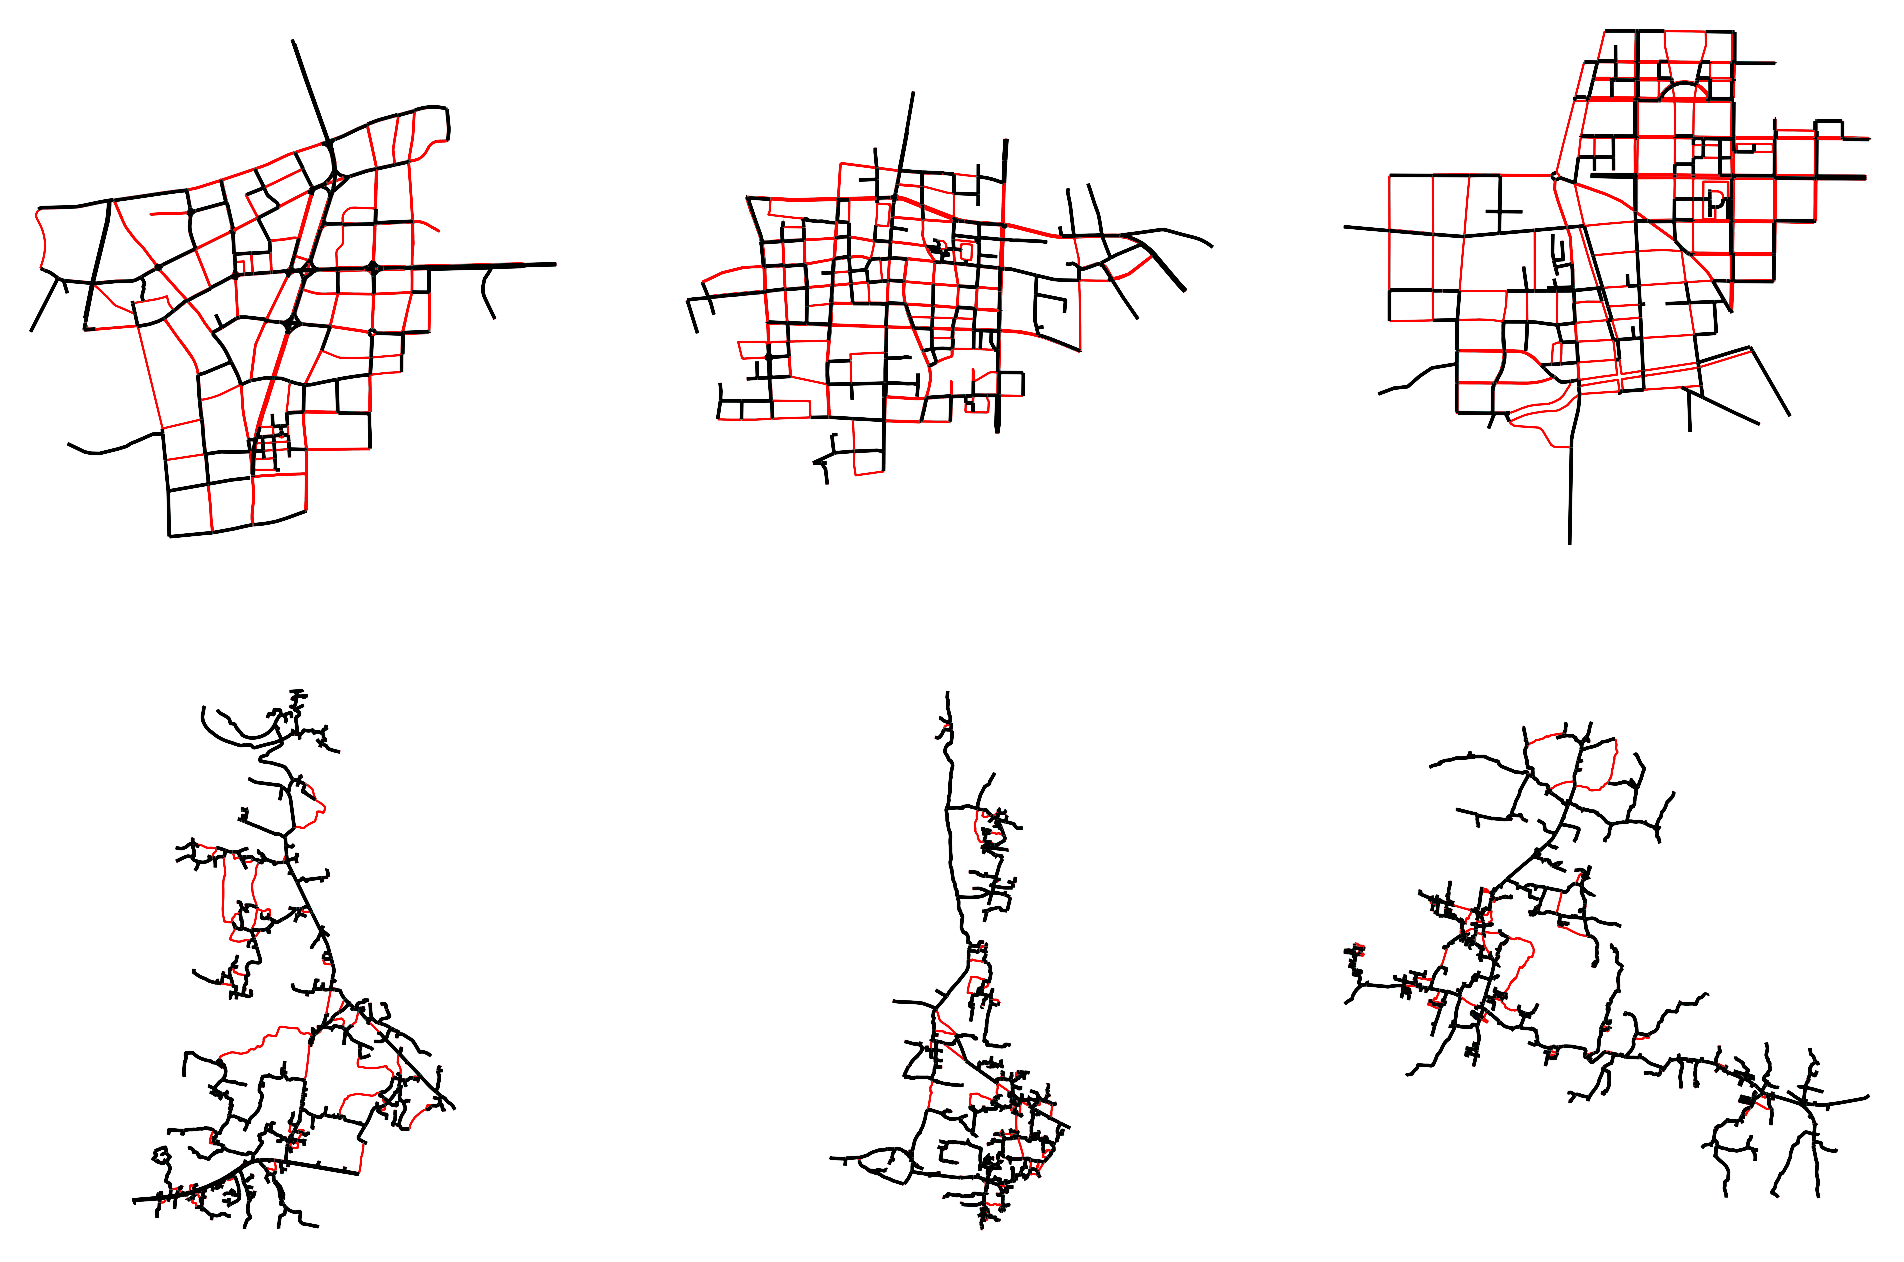
\includegraphics[width=0.90\textwidth]{fig_network_examples.png}
    \caption{Example small city street networks. Black lines represent the MST and red lines represent the rest of the full network. Top row: low treeness/high redundancy. Bottom row: high treeness/low redundancy.}\label{fig:network_examples}
\end{figure*}

One such topological indicator of this treeness could be the \textit{link redundancy}, akin to a normalized version of what in graph theory is called the circuit rank (the rank of the graph's first homology group): the count of how many edges must be removed to reduce a graph to a spanning tree \citep{xie_2007_measuring}. This would measure how tree-like the network is in terms of how many structurally redundant links exist beyond those necessary to uniquely connect the nodes \citep{buhl_2006_topological}. However, this is purely topological and ignores the spatially-embedded geometry of spatial graphs like street networks. A geometric equivalent could be the \textit{length redundancy}, which measures the share of the full network's total length that is in excess of the MST. This would indicate how much extra infrastructure was built beyond the minimum necessary to connect the city.

\subsection{Are Some Cities Trees?}

Many geographical systems are trees, including natural systems like river networks and artificial systems like municipal stormwater drainage piping \citep{hesarkazzazi_assessing_2020,sanchirico_river_2025}. The latter suggests that certain physical urban infrastructure could be tree-like due to costs or efficiency. Given that, are some cities' street networks actually (or nearly) trees?

Transportation scholars have considered urban street networks as trees to distinguish branching structures from circuit-based networks. \citet{xie_2007_measuring} define road-network treeness as the complement of arterial circuitness, distinguishing tree-like arterial systems from ring, web, and beltway forms. \citet{levinson_2012_network} applies a related empirical measure to U.S. metropolitan areas, defining treeness as the share of total street length that belongs to branches rather than circuits. \citet{han_2020_classification} classify urban street networks by tree-like features such as T-intersections, cul-de-sacs, penetrating streets, and cells. Together, this literature treats treeness as a measurable street network property, but mainly through arterial structure, branch/circuit classification, or local design features.

This raises a broader theoretical question: if treeness is measurable, what does it mean for a spatial infrastructure network? Spatial network science treats trees as the minimum connected infrastructure against which redundancy, efficiency, and robustness can be evaluated. \citet{buhl_2006_topological} place self-organized street networks between tree structures and planar triangulations, finding that tree-like settlements are more vulnerable while meshed forms are more robust and efficient. \citet{cardillo_2006_structural} compare urban street samples to minimum spanning trees and greedy triangulations, interpreting real street networks as occupying a cost-efficiency space between minimally and highly connected planar forms. \citet{barthelemy_2022_spatial} formalizes this broader trade-off in spatial networks: links added beyond a minimum spanning tree raise infrastructure cost while improving accessibility, efficiency, and fault tolerance.

These trade-offs matter for urban planning and geography because street network treeness shapes how cities function. \citet{huang_city_2022} revisit Alexander's conjecture empirically, relating meshedness and other street-network indicators to urban life across multiple cities. \citet{barringtonleigh_2019_global} measure street-network disconnectedness worldwide and classify networks across forms ranging from grids to dendritic (i.e., tree-like) and circuitous layouts. \citet{boeing_2024_resilient} shows that disruption vulnerability is lower in street networks with more connectivity, less dependence on chokepoints, and more direct routes.

The prior literature therefore establishes treeness as theoretically and practically important, and treeness indicators could thus quantify the vulnerability and (inverse) redundancy of urban street networks around the world. However, this literature remains limited by small samples, regional scope, narrow measures, typological proxies, or indirect indicators such as meshedness and disconnectedness. This leaves our central empirical question open: how tree-like are cities around the world?

\section{Methods}

This study addresses this and asks: to what extent are cities' street networks tree-like? We model the street networks of every urban area in the world then find each's MST to measure its link redundancy and length redundancy. Here we describe our data sources, calculations, and analyses, including baseline comparisons and robustness checks.

\subsection{Data Sources}

We use the models of the street networks of every urban area in the world from \citet{boeing_urban_2026}. These are 10,351 undirected graphs where nodes represent intersections/dead-ends and edges represent street segments \citep{boeing_topological_2025}. Each graph edge has a weight attribute representing its length in meters. We use undirected graphs because active transportation such as walking is undirected, as is the underlying infrastructure itself, even if certain vehicles face flow direction constraints on some streets.

\subsection{Measuring Treeness}

For each of these urban area street networks, let $G$ be the full network's undirected graph and let $T$ be its length-weighted MST (or minimum spanning forest if $G$ is not fully connected, as discussed below). We compare $G$ to $T$ via link redundancy and length redundancy.

First we define the link redundancy, $\theta$, as:

\begin{equation}
    \label{eq:link_redundancy_1}
    \theta = \frac{m - n + c}{m}
\end{equation}

where $m$ and $n$ are as defined in \autoref{sec:theory_network_treeness} and $c$ is $G$'s component count ($c = 1$ if $G$ is fully connected, higher if not). The numerator represents the aforementioned circuit rank and the denominator normalizes it. Note that \autoref{eq:link_redundancy_1} could be equivalently expressed as:

\begin{equation}
    \label{eq:link_redundancy_2}
    \theta = 1 - \frac{m_T}{m}
\end{equation}

where $m_T$ is the number of edges in $T$. As redundancy and connectedness are somewhat related conceptually, we can test the relationship between $\theta$ and the average node degree, $\langle k \rangle$, a common measure of graph connectedness defined as:

\begin{equation}
    \label{eq:avg_node_degree}
    \langle k \rangle = \frac{2m}{n}
\end{equation}

$\theta$ also shares some conceptual similarity with the normalized meshedness coefficient, $\alpha$, which appears in transport engineering and is the ratio of a connected graph's circuit rank to the maximum possible number of cycles in a planar graph with the same node count \citep{levinson_2012_network,buhl_2006_topological,cardillo_2006_structural}:

\begin{equation}
    \label{eq:meshedness_coefficient}
    \alpha = \frac{m - n + 1}{2 n - 5}
\end{equation}

where the denominator derives from algebraic homology's Euler characteristic of planar graphs, since urban street networks are quasiplanar \citep{boeing_planarity_2020}. However, by combining Equations \ref{eq:avg_node_degree} and \ref{eq:meshedness_coefficient} we can see that, as $n \to \infty$,

\begin{equation}
    \label{eq:alpha_to_infinity}
    \alpha \to \frac{\langle k \rangle}{4} - 0.5
\end{equation}

Thus, for large graphs like urban-scale street networks, $\alpha$ is approximately an affine transformation of $\langle k \rangle$ and therefore offers minimal statistical information beyond $\langle k \rangle$ itself. This makes the link redundancy, $\theta$, a more useful topological indicator of redundancy and (inverse) treeness for comparison across city-sized street networks.

Moving beyond pure topology, we also calculate a geometric indicator---the length redundancy, $\lambda$---as a geometric corollary to $\theta$. It represents the share of the full network's length in excess of the MST's length and is defined as:

\begin{equation}
    \label{eq:length_redundancy}
    \lambda = 1 - \frac{L_T}{L}
\end{equation}

where $L_T$ is as defined in \autoref{eq:total_edge_length} and $L$ is the equivalent total length of $G$. Note the mathematical correspondence between Equations \ref{eq:link_redundancy_2} and \ref{eq:length_redundancy}. Both $\theta$ and $\lambda$ are bounded by $[0,1)$, assuming $m > 0$ and $L > 0$ for any nontrivial real-world network. These are both indicators of treeness since $\theta = \lambda = 0$ indicates a perfect tree and higher values indicating greater redundancy/less treeness.

\subsection{Analysis}
\label{sec:methods_analysis}

We calculate these treeness indicators for every urban area in the world then analyze their distributions to describe the nature of urban treeness. We also calculate Pearson correlation coefficients to test their relationships with each other and with other urban indicators from \citet{boeing_urban_2026}, which describes the latter in detail. They include the aforementioned total network length $L$ (meters), hilliness (the standard deviation of node elevations, meters), the aforementioned average node degree $\langle k \rangle$ (dimensionless), the Gini coefficient of node betweenness centralities (a dimensionless measure of concentrated importance in certain nodes), average circuity (a dimensionless measure of the streets' deviation from straight lines), orientation entropy (a dimensionless measure of the disorder in street bearings), built-up area (km\textsuperscript{2}), intersection density (per km\textsuperscript{2} of built-up area), and population density (1000s of persons per km\textsuperscript{2} of built-up area). We take the natural logarithms of $L$ and built-up area for a better linear fit.

\subsection{Baselines and Robustness Checks}

To establish an empirical baseline, we also calculate $\theta$ for several other kinds of undirected networks available from the ICON\endnote{Available online at \url{https://icon.colorado.edu/}} database, including the MSN social network \citep{leskovec_planetary-scale_2008}, the European airline network \citep{cardillo_emergence_2013}, the Paris subway network \citep{roth_long-time_2012}, and the Delhi bus route network \citep{chatterjee_statistical_2016}. To do so, we use the $m$ and $n$ values reported in each reference and assume $c=1$, which introduces a merely negligible error when the number of components is small relative to $m$, as is normal. These baselines are not experimental controls or matched counterfactuals and they differ in spatial embedding, planarity, and scale. We use them only as reference points to contextualize the magnitude and range of urban street network treeness relative to other familiar network types.

We also conduct two robustness checks by recalculating $\theta$ and $\lambda$ for (1) a topologically corrected version of $G$, and (2) only the largest component of $G$. For the first, we topologically correct $G$ using the \texttt{neatnet} package \citep{fleischmann_adaptive_2026}. This simplifies complex digitization, for example by collapsing multiple nodes representing single real-world intersections or multiple edges representing centerlines of a single divided road. This tests whether excess edges arising merely as artifacts of digitization bias our results by making networks appear more redundant than they actually are.

Regarding the second, urban street networks are usually fully connected in the real world: you can reach any node from any other node. However, controlled access points, ferries, and the imposition of an artificial perimeter on the graph can produce disjoint components. If this happens, the MST of the full graph is technically a minimum spanning forest instead, and $\theta$ will be biased upward by the number of components, $c$, in the graph: per \autoref{eq:link_redundancy_1}, as $c$ increases, $\theta$ increases even if the actual redundancy of the network has not changed. Therefore, we recalculate $\theta$ and $\lambda$ for each graph's largest component only, to test whether disconnected graphs bias our results.

\section{Findings}

\subsection{Empirical Baselines}\label{sec:findings_empirical_baselines}

We first report the $\theta$ values calculated for the other \enquote{kinds} of networks as a baseline. The MSN social network---an aspatial network---has a $\theta$ of 0.862. The European airline network---a spatial network with nodes but not edges embedded in space---is 0.875. The Paris subway network---a spatial network with both nodes and edges embedded in space---is 0.581, and the Delhi bus route network---another spatial network with both nodes and edges embedded in space---is 0.638. In other words, we can interpret these baselines as indicating that 58--88\% of these networks' edges would have to be removed to reduce them to their spanning trees.

\subsection{Empirical Street Network Treeness}

\autoref{tab:treeness_descriptive} presents descriptive statistics for our two indicators of treeness. Across all the world's urban areas, the link redundancy, $\theta$, ranges empirically from 0.031--0.458 with a mean of 0.281, a median of 0.288, and a standard deviation of 0.068. This indicates that only 28\% of the edges in the average urban street network would have to be removed to reduce it to its spanning tree. In fact, the maximum observed $\theta$ of 0.458 means that there is no street network in the world that even approaches the baseline $\theta$ values of the other kinds of networks reported in \autoref{sec:findings_empirical_baselines}. That is, \textit{every} urban street network in the world is more tree-like than those baseline networks are.

\begin{table*}[!tb]
    \footnotesize
    \centering
    \caption{Descriptive statistics for the street network treeness indicators, $\theta$ (link redundancy) and $\lambda$ (length redundancy), across all of the world's urban areas and broken out by geographical sub-region.}\label{tab:treeness_descriptive}
\begin{tabular}{lrrrrrrrr}
\toprule
 & \multicolumn{4}{c}{Link Redundancy ($\theta$)} & \multicolumn{4}{c}{Length Redundancy ($\lambda$)} \\
 & Min & Mean & Median & Max & Min & Mean & Median & Max \\
\midrule
Australia/New Zealand & 0.176 & 0.257 & 0.256 & 0.327 & 0.309 & 0.429 & 0.432 & 0.526 \\
Central/Southern Asia & 0.031 & 0.231 & 0.236 & 0.428 & 0.024 & 0.380 & 0.387 & 0.707 \\
Eastern/SE Asia & 0.062 & 0.295 & 0.308 & 0.436 & 0.132 & 0.453 & 0.465 & 0.675 \\
Europe & 0.070 & 0.264 & 0.276 & 0.382 & 0.166 & 0.428 & 0.439 & 0.599 \\
Lat. Am./Caribbean & 0.109 & 0.327 & 0.337 & 0.458 & 0.178 & 0.498 & 0.509 & 0.692 \\
N Africa and W Asia & 0.077 & 0.305 & 0.317 & 0.432 & 0.183 & 0.488 & 0.503 & 0.601 \\
Northern America & 0.175 & 0.299 & 0.304 & 0.392 & 0.303 & 0.484 & 0.491 & 0.601 \\
Oceania & 0.095 & 0.182 & 0.197 & 0.277 & 0.186 & 0.305 & 0.335 & 0.447 \\
Sub-Saharan Africa & 0.083 & 0.290 & 0.296 & 0.449 & 0.113 & 0.441 & 0.451 & 0.637 \\
\midrule
Worldwide & 0.031 & 0.281 & 0.288 & 0.458 & 0.024 & 0.442 & 0.454 & 0.707 \\
\bottomrule
\end{tabular}
\end{table*}

Similarly, the length redundancy, $\lambda$, ranges empirically from 0.024--0.707 with a mean of 0.442, a median of 0.454, and a standard deviation of 0.091. This indicates that 44\% of the edge length in the average urban street network would have to be removed to reduce it to its spanning tree. As expected, we see that $\lambda$ is typically higher than $\theta$ (since $T$ is a length-weighted MST) but they are strongly correlated ($r = 0.90$, $p < 0.001$), indicating a close relationship between topological and geometric treeness.

\begin{figure*}[!tb]
    \centering
    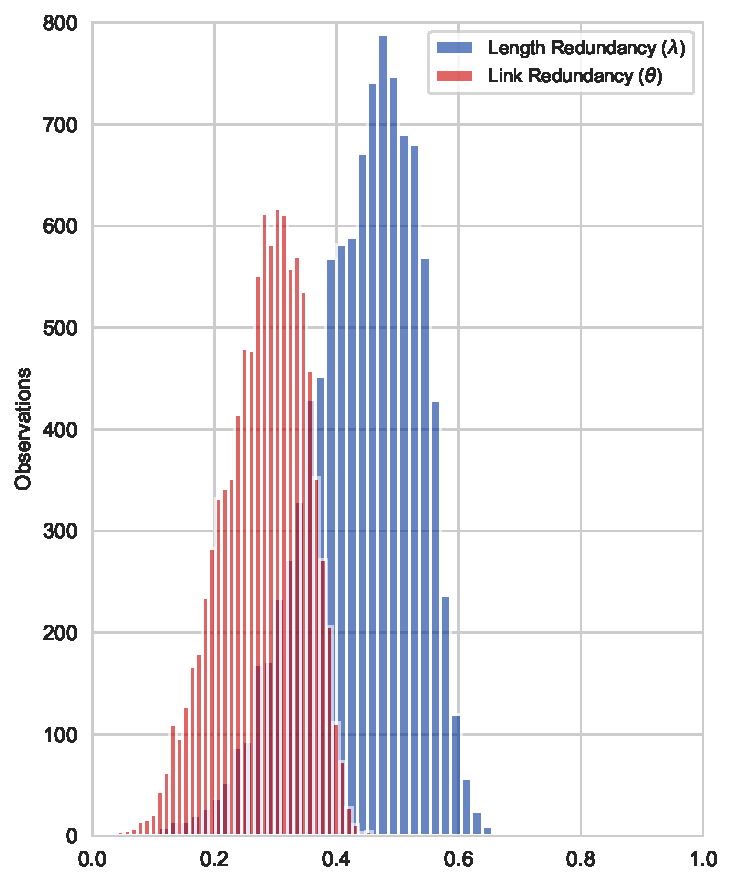
\includegraphics[width=0.50\textwidth]{fig_histogram_indicators.pdf}
    \caption{Histograms of the statistical distributions of the street network treeness indicators, $\theta$ (link redundancy) and $\lambda$ (length redundancy), across all of the world's urban areas.}\label{fig:histogram_indicators}
\end{figure*}

\begin{figure*}[!tb]
    \centering
    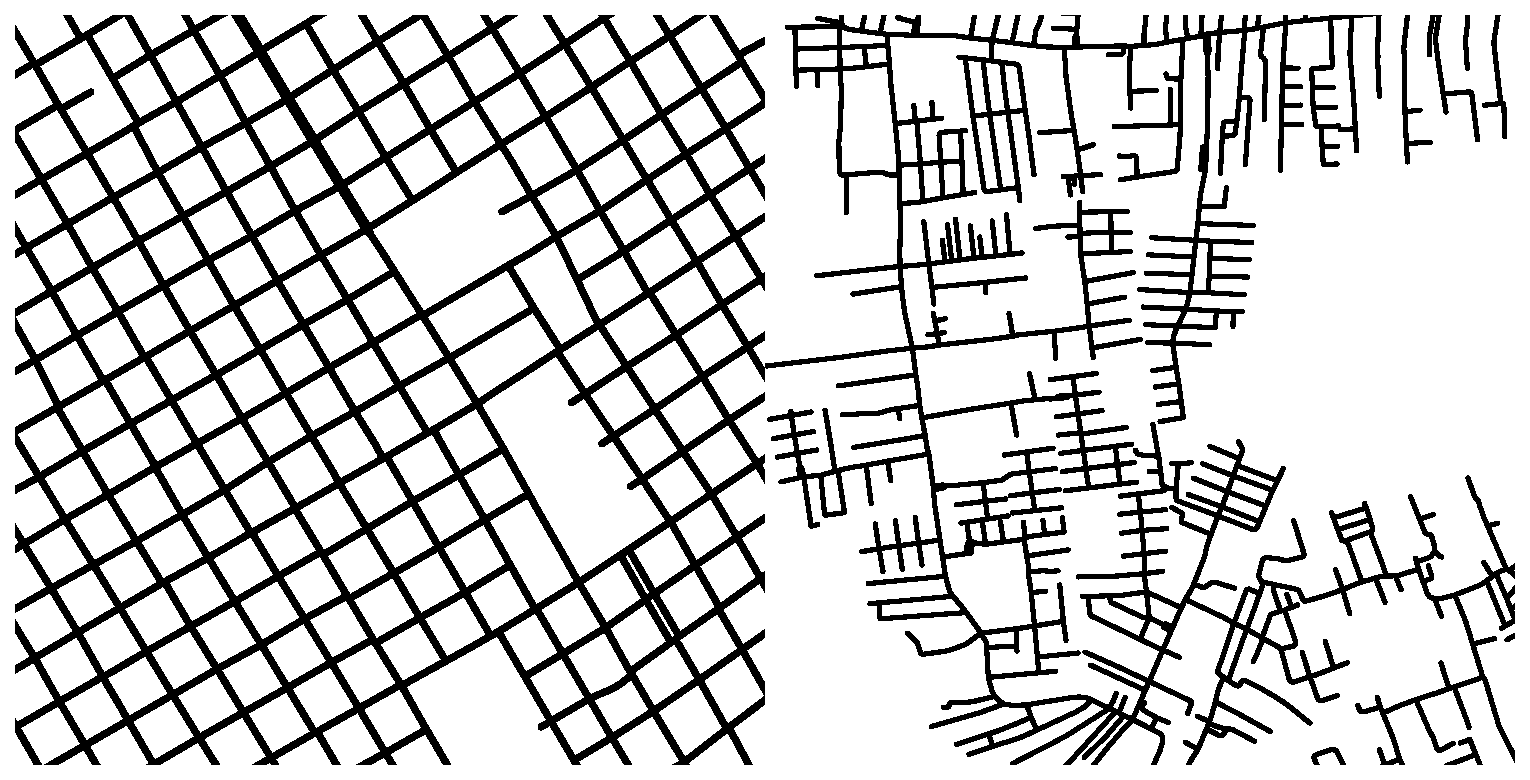
\includegraphics[width=0.90\textwidth]{fig_ba_vs_bangkok.pdf}
    \caption{Example street networks: one-square mile of Buenos Aires (left, low treeness) and Bangkok (right, high treeness.)}\label{fig:ba_vs_bangkok}
\end{figure*}

\begin{figure*}[!tb]
    \centering
    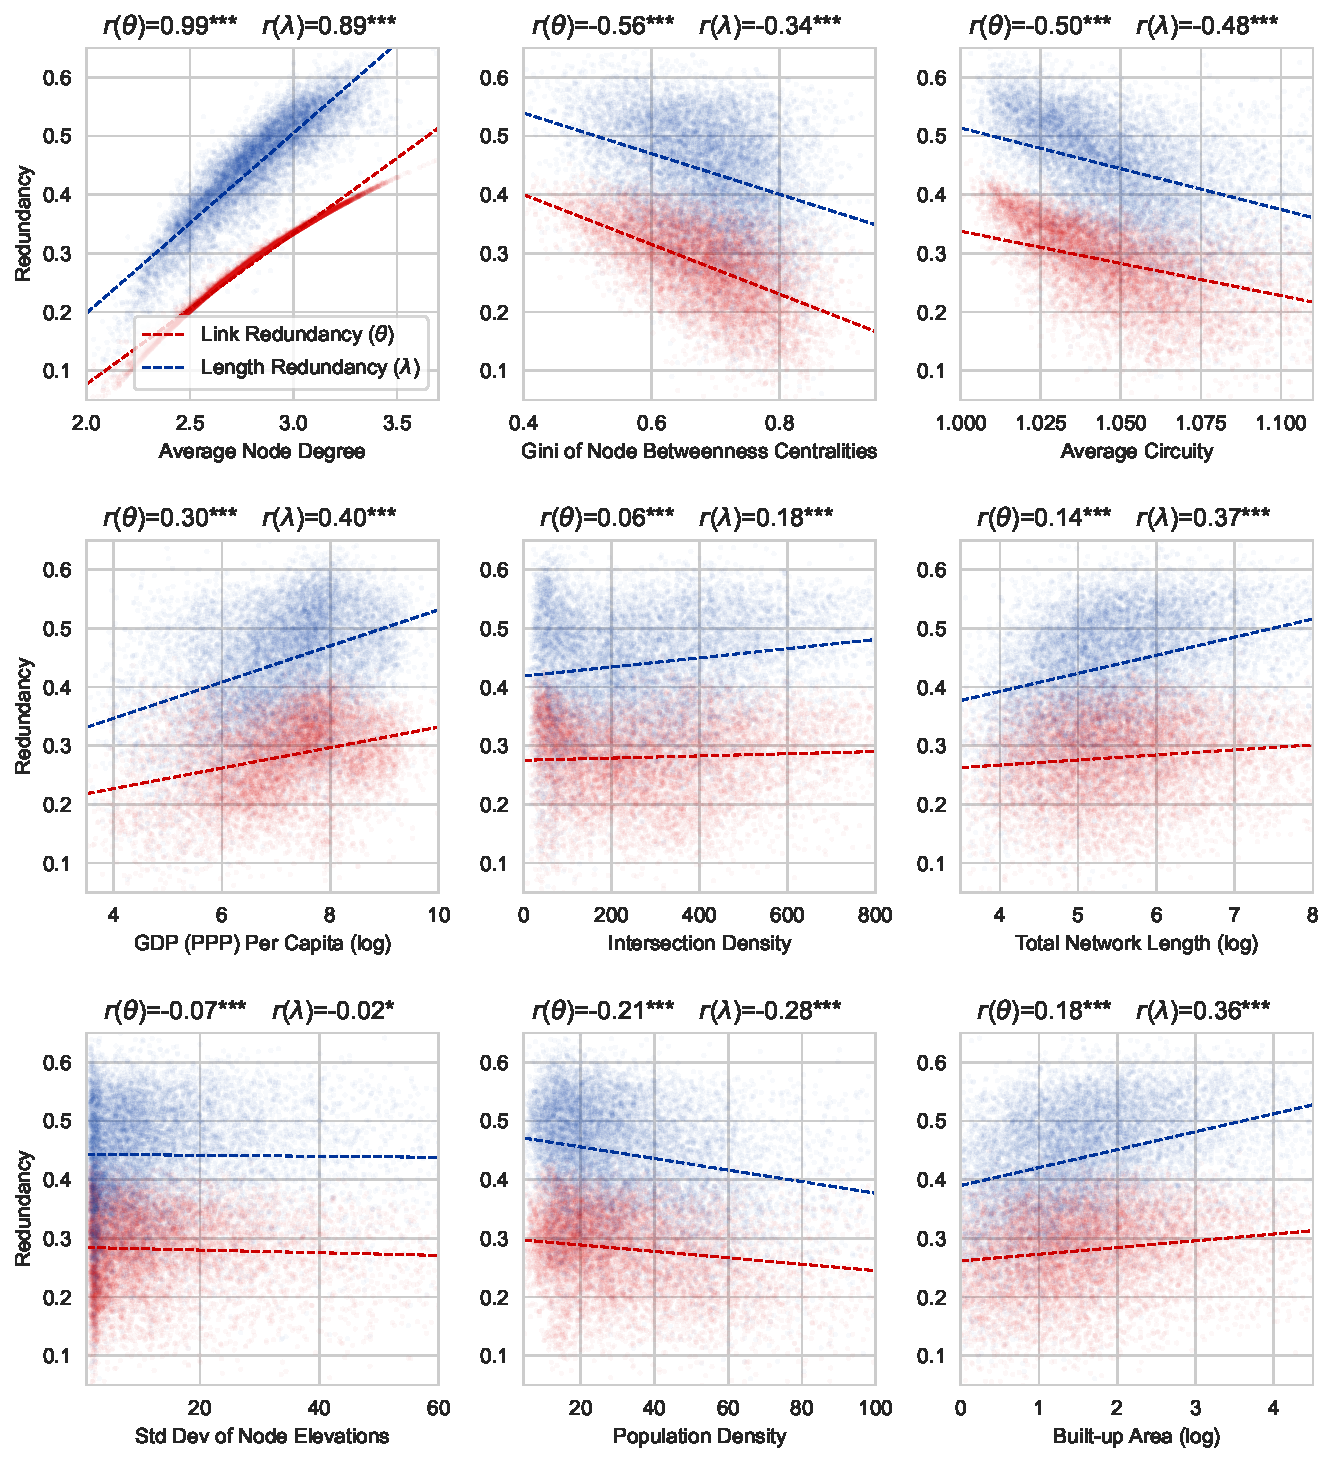
\includegraphics[width=1\textwidth]{fig_scatter_regressions.pdf}
    \caption{Relationships between $\theta$ (link redundancy), $\lambda$ (length redundancy), and other variables across all of the world's urban areas (units described in \autoref{sec:methods_analysis}). Correlation coefficients ($r$) are shown with statistical significance (* $p < 0.05$, *** $p < 0.001$).}\label{fig:scatter_regressions}
\end{figure*}

\autoref{fig:histogram_indicators} illustrates the statistical distributions of $\theta$ and $\lambda$ across all the urban areas. It reveals a particularly interesting property of urban treeness: there is little heterogeneity around the world. Both histograms are sharply peaked with narrow tails, no outliers, and little statistical variation: in fact, their coefficients of variation ($\sigma$ / $\mu$) are just 0.242 ($\theta$) and 0.205 ($\lambda$). These are bounded indicators, but most observations cluster fairly tightly around the mean. In other words, the treeness of urban street networks has a characteristic scale despite the scale-invariance of city size and the wide variety of urban forms and contexts.

In spite of this characteristic scale, there are some differences in different parts of the world (\autoref{tab:treeness_descriptive}). For example, Latin American and Caribbean cities have the highest mean $\theta$ and $\lambda$ values, while Oceania has the lowest. However, except for Oceania, all regions' means fall within one standard deviation of both indicators' worldwide means. Among megacities with at least 10 million residents, Buenos Aires is the least tree-like urban area ($\theta=0.415$, $\lambda=0.555$) and Bangkok is the most ($\theta=0.131$, $\lambda=0.290$). The characteristic one square mile segments of each in \autoref{fig:ba_vs_bangkok} helps illustrate why: Buenos Aires has a lattice-like grid across the city, whereas Bangkok's network epitomizes a tree with its dendritic, branching dead-ends.

\autoref{fig:scatter_regressions} shows that both $\theta$ and $\lambda$ have statistically significant relationships with all the other urban variables. For example, both strongly and positively correlate with $\langle k \rangle$, indicating that more-connected networks are less tree-like, which is expected given the mathematical expressions of these measures. Both moderately and negatively correlate with the Gini coefficient of node betweenness centralities, indicating that more tree-like networks are more prone to node importance being heavily concentrated in certain nodes. Both moderately and negatively correlate with average circuity, indicating that more tree-like networks tend to be more geometrically circuitous/less efficient. They moderately and negatively correlate with orientation entropy, indicating that more tree-like networks are less consistently grid-like in their street bearings. Both $\theta$ (weakly) and $\lambda$ (moderately) positively correlate with both $L$ and built-up area, indicating that larger cities---in terms of total street length or urban area size---tend to be less tree-like. Both weakly correlate with intersection density (positively) and population density (negatively), indicating that more tree-like cities have sparser intersection densities but denser resident populations. Finally, both weakly but negatively correlate with the standard deviation of node elevations, indicating that hillier cities tend to be more tree-like.

\subsection{Robustness Checks}

We observe that our empirical findings are robust against re-analyzing the topologically corrected graphs. For example, the global mean $\theta$ drops only slightly from 0.28 to 0.26 and mean $\lambda$ drops from 0.44 to 0.41, as expected since topological correction should remove at least some edges. The relationships in \autoref{fig:scatter_regressions} remain stable, with the same signs and similar magnitudes. When re-analyzing only the largest component, we observe even greater robustness of the findings. The global mean $\theta$ remains 0.28 and mean $\lambda$ remains 0.44. Again the relationships in \autoref{fig:scatter_regressions} remain stable, with the same signs and similar magnitudes. In fact, in the median urban area, 99.8\% of the edges belong to the largest component. Overall, these checks show that our findings are unbiased by digitization artifacts or disconnected graphs.

\section{Discussion}

\subsection{A City Is Sometimes Kind of a Tree}

This suggests that urban treeness is a fundamental property of cities that is relatively invariant across the world, despite the wide variety of urban forms and contexts. This also suggests that there may be some underlying universal processes or constraints that shape urban treeness, which we theorize in the next section.

\subsection{Treeness and Redundancy in Urban Form}

TBD

\section*{Acknowledgments}

I wrote this paper myself, by hand, without AI:\@ the ideas and any mistakes are my own. Early portions of this research-in-progress were presented in (far too many) talks at Harvard University, the London School of Economics, UCL CASA, the University of Liverpool, New York University, the University of Pennsylvania, the Complexity Science Hub in Vienna, Charles University in Prague, the University of Zurich, the ISI Foundation in Turin, and the University of Helsinki. I am grateful for all the helpful feedback from these audiences that helped me shape these ideas. Sabbaticals are a good thing.

% print the footnotes as endnotes, if any exist
\IfFileExists{\jobname.ent}{\theendnotes}{}

% print the bibliography
\setlength{\bibsep}{0.00cm plus 0.05cm} % no space between items
\bibliographystyle{apalike}
\bibliography{references}

\end{document}
